\documentclass{article}

\usepackage[final]{neurips_2019}

\usepackage[utf8]{inputenc}
\usepackage[T1]{fontenc}
\usepackage{hyperref}
\usepackage{url}
\usepackage{booktabs}
\usepackage{amsfonts}
\usepackage{amsmath}
\usepackage{nicefrac}
\usepackage{microtype}
\usepackage{graphicx}
\usepackage{float}
\usepackage{xcolor}
\usepackage{lipsum}

\newcommand{\note}[1]{\textcolor{blue}{{#1}}}

\title{
  Invariance and Generalization in Sharpness-Aware Minimization (SAM)-Variants \\
  \vspace{1em}
  \small{\normalfont Stanford CS229 Project}  % Select one and delete the other
}

\author{
  Manav Dahra \\
  Department of Computer Science \\
  Stanford University \\
  \texttt{mav3rik@stanford.edu} \\
  % Examples of more authors
%   \And
%   Name \\
%   Department of Computer Science \\
%   Stanford University \\
%   \texttt{name@stanford.edu} \\
%   \And
%   Name \\
%   Department of Computer Science \\
%   Stanford University \\
%   \texttt{name@stanford.edu}
}

\begin{document}

\maketitle

\begin{abstract}
In this study we train ResNet-18 \& ViT-B/32 architectures under reparametrized settings using different variants of SAM optimizers. We compare their loss landscape curvature, generalisation gap and rate of convergence to find that overall, Monge-SAM performs the best across these metrics.
\end{abstract}


% {\color{red} This template does not contain the full instruction set for this assignment; please refer back to the milestone instructions PDF.

\section{Introduction}

\subsection{Motivation}

Recently, Sharpness-Aware Minimization (SAM) method and its variants have been proposed which use local perturbations at each optimization step to steer networks into flatter loss regions. Across these variants, the exact methodology of computing perturbations varies from relying on Euclidean metric for perturbation radius to using scale invariance and geometry-aware metrics. And even though these methods have shown theoretical and empirical improvements on generalization, they require a systematic empirical comparison under controlled settings. Additionally, each optimisation step in these methods require multiple forward and backward passes, which can be computationally expensive. It raises questions about the practical trade-offs between improved generalization and increased training time, especially for larger models and datasets.

This motivates our study to empirically validate some of these concepts by running extensive experiments on ResNet-18 and ViT-B/32 architectures using CIFAR-10 dataset as the input and predicted labels as the output. We focus on comparing how modern optimization paradigms, specifically SAM, Adaptive SAM (ASAM) and Monge SAM (M-SAM) actually withstand explicit parameter distortions against SGD optimizer.

\section{Related Work}

\subsection{Background}

The relationship between the geometry of the loss landscape and a model's generalization capacity has been a topic of interest in deep learning optimization research, fundamentally dating back to the concept of flat minima introduced by \citet{hochreiter1997flat} and expanded by \citet{keskar2016large}. However, \citet{dinh17b} demonstrated a critical flaw in traditional Euclidean metrics, proving that standard measures of flatness are highly sensitive to function-preserving reparametrizations. This was shown by doing node-rescaling in ReLU networks, meaning a minimum can be rendered arbitrarily sharp without altering its generalization behavior. 

This insight revealed that the commonly held belief that flat minima inherently generalize better than sharp minima is not universally valid, as the notion of flatness can be manipulated through reparametrization. This has significant implications for optimization algorithms that rely on Euclidean metrics to find flat minima, as they may be misled by the geometry of the parameter space rather than the true generalization properties of the model.

To address this limitation and actively seek flatter regions, researchers have developed optimization algorithms over the years which can be broadly categorized into following paradigms:

\textbf{Traditional Euclidean Sharpness-Aware Methods (SAM):}

\citet{foret2021sam} introduced Sharpness-Aware Minimization (SAM), which augments SGD with a two-step update: parameters are first perturbed to the approximate local loss maximum within an $\ell_2$ ball of radius $\rho$, then a standard gradient step is taken at the perturbed point. The key idea is to minimise the worst-case loss within a small neighbourhood, avoiding the prohibitively expensive Hessian. Since the perturbation ball is Euclidean it is \emph{not} invariant to function-preserving rescalings of the weights, inheriting the vulnerability identified by \citet{dinh17b}.

\textbf{Scale-Invariant Sharpness-Aware Methods (ASAM):}

To address the scale-sensitivity of SAM, \citet{kwon2021asam} replaces the $\ell_2$ ball with a parameter-scaled adaptive ball, making the perturbation invariant to element-wise weight rescaling. This is computationally lightweight, but the diagonal scaling operator $T_w = \mathrm{diag}(|w|+\eta)$ assumes all parameters are statistically independent, which may not hold in practice.


\textbf{Geometry-Aware Sharpness-Aware Methods (Monge SAM):}

The current SOTA paradigm treats the parameter space as a curved Riemannian manifold. \citet{jacobsen2025msam} equip it with the \emph{Monge metric} $G(\theta) = I_K + \nabla\ell(\theta)\nabla\ell(\theta)^\top$, induced by embedding the loss surface as a graph in $\mathbb{R}^{K+1}$. This captures full inter-parameter correlations via the loss gradient, without requiring a probabilistic model formulation. See Table~\ref{tab:perturbations} for the resulting perturbation.

However, existing empirical validations of M-SAM are highly limited, restricted entirely to a narrow fine-tuning task on a pre-trained ResNet-18 and a multi-modal alignment task.

\textbf{The Empirical Bridge:} While these subsequent iterations offer robust theoretical guarantees for reparametrization invariance, existing empirical validations remain fragmented, lacking a systematically controlled reparametrization benchmark across diverse, modern neural architectures like Convolutional Networks and Vision Transformers. Our study unifies all three optimization paradigms into a highly controlled, multi-factorial grid—sweeping across architectures (ResNet-18 vs. ViT), initialization scales (\(1.0\) vs. \(5.0\)), perturbation radii (\(\rho \in \{0.05, 0.1, 0.5\}\)), and multiple random seeds (\(40, 41, 42\)). This comprehensive empirical framework allows us to directly compare the optimizers' performance under explicit reparametrization distortions, providing a clearer picture of their practical robustness and generalization capabilities.

\section{Dataset and Features}

\textbf{Dataset.} We use CIFAR-10 \citep{Krizhevsky09learningmultiple}, loaded via the HuggingFace Datasets library \citep{lhoest-etal-2021-datasets}. It consists of 60{,}000 colour images across 10 balanced classes (airplane, automobile, bird, cat, deer, dog, frog, horse, ship, truck). We use the standard split: \textbf{50{,}000 training} and \textbf{10{,}000 test} images. No separate validation set is held out; early-stopping decisions are based on test accuracy after each epoch.

\textbf{Input/Output.} The input to each model is a pre-processed $3 \times H \times W$ image tensor; the output is a predicted class label from the 10 CIFAR-10 categories.

\textbf{Preprocessing and augmentation.} Raw images are $32 \times 32$ pixels. For ResNet-18 we keep the native resolution; for ViT-B/32 we upsample to $224 \times 224$ (the resolution expected by the pre-trained patch embedding). All images are normalised channel-wise using the per-channel empirical mean and standard deviation computed over the training set. During training we apply standard data augmentation: random crop with padding 4 and random horizontal flip. No augmentation is applied at test time beyond resizing and normalisation. See Appendix~\ref{appendix:preprocessing} for more details.

\textbf{Features.} We feed raw pixel values directly into the networks; no hand-crafted feature extraction (e.g.\ HOG, SIFT) is used. ResNet-18 learns hierarchical convolutional features from scratch on CIFAR-10, while ViT-B/32 is fine-tuned from ImageNet pre-trained weights and processes the image as a sequence of $32 \times 32$ non-overlapping patches projected into a 768-dimensional embedding space.

\textbf{Reparametrisation setup.} To evaluate optimizer robustness, we introduce explicit weight distortions at initialisation by scaling all parameters by a factor $\alpha \in \{1.0,\, 5.0\}$. A scale of $\alpha=1.0$ is the standard baseline; $\alpha=5.0$ represents an adversarially sharp initialisation that exposes the scale-sensitivity of Euclidean perturbation methods.

\begin{figure}[H]
    \centering
    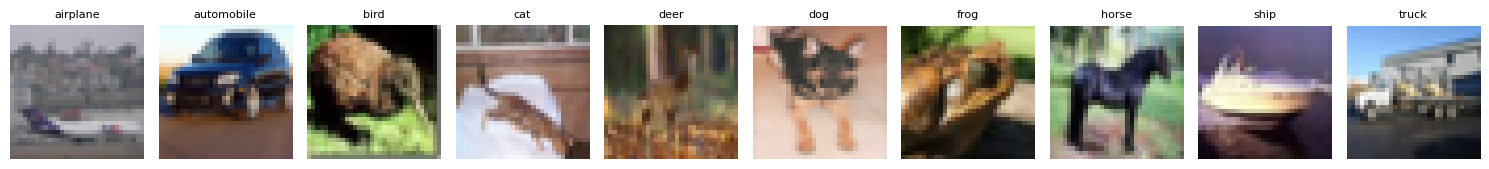
\includegraphics[width=\textwidth]{./cifar10_samples.png}
    \caption{Example images from the CIFAR-10 dataset (one per class). Classes are, from left to right: airplane, automobile, bird, cat, deer, dog, frog, horse, ship, truck.}
    \label{fig:cifar10_samples}
\end{figure}

\section{Methods}
Describe your learning algorithms, proposed algorithm(s), or theoretical proof(s). Make sure to include relevant mathematical notation. For example, you can briefly include the SVM optimization objective/formula or say what the softmax function is. It is okay to use formulas from the lecture notes. For each algorithm, give a short description (\~ 1 para- graph) of how it works. Again, we are looking for your understanding of how these machine learning algorithms work. Although the teaching staff probably know the algorithms, future readers may not (reports will be posted on the class website). Additionally, if you are using a niche or cutting-edge algorithm (e.g. long short-term memory, SURF features, or anything else not covered in the class), you may want to explain your algorithm using 1/2 paragraphs. Note: Theory/algorithms projects may have an appendix showing extended proofs (see Appendix section below).

\subsection{Experimental setup}
Our experiment is split into following stages:
\begin{itemize}
    \item \textbf{Baseline.} Run a standard training loop that sweeps across a grid of hyper-parameters without any reparametrization (i.e. $\alpha=1.0$) to establish a baseline performance. For complete details of hyper-parameters see Appendix~\ref{appendix:hyperparameters}. The training loop also  generates trained checkpoints and key metrics like loss, accuracy and elapsed time for all epochs and seeds. 
    \item \textbf{Reparameterisation.} Next, we introduce reparametrization by scaling initial weights with $\alpha=5.0$ and repeat the training loop for same hyper-parameter grid. This allows us to directly compare how each optimizer's performance changes under explicit weight distortions, revealing their robustness to sharp initializations.
    \item \textbf{Analysis.} Next, we analyse collected results to compare optimizers across multiple dimensions: convergence speed, final test accuracy, generalization gap (train vs. test accuracy), and loss landscape curvature using Hutchinson's trace estimation. We also visualise training curves and loss landscapes to qualitatively assess optimizer behavior under reparametrization.
\end{itemize}

\subsection{Reparameterisation setup ResNet vs ViT}

For ResNet-18 each BasicBlock has the following computation chain:
\[
  \hdots 
  \xrightarrow{\text{conv1}} 
  \xrightarrow{\text{BN1}} 
  \xrightarrow{\text{ReLU}}
  \xrightarrow{\text{conv2}} 
  \xrightarrow{\;\times 1/\alpha\;} 
  \xrightarrow{\text{BN2}} 
  \hdots
\]

we can reparametrize it by injecting a positive scaling factor $\alpha$ at Batch normalisation layer (BN1) and compensating with $1/\alpha$ at Convolution layer (conv2), yielding the following chain which preserves the function computed by the block. See Appendix~\ref{appendix:reparametrization} for more details.
\[
  \hdots 
  \xrightarrow{\text{conv1}} 
  \xrightarrow{\text{BN1}} 
  \xrightarrow{\;\times\alpha\;} 
  \xrightarrow{\text{ReLU}} 
  \xrightarrow{\text{conv2}} 
  \xrightarrow{\;\times 1/\alpha\;} 
  \xrightarrow{\text{BN2}} 
  \hdots
\]

For ViT-B/32, we apply reparameterisation in the MLP layers of the transformer blocks. Each transformer block contains multi-head self-attention and feedforward layers, with GELU activations. Since GELU activation used in ViT-B/32 is not positively homogeneous, meaning it does not satisfy $f(\alpha x) = \alpha f(x)$ for all $\alpha > 0$. This means that simply scaling the weights by $\alpha$ does not correspond to a function-preserving reparametrization, as the output of the GELU activation will not scale linearly with the input. To get around this issue, we patch the GELU activation function by its first-order Taylor expansion around zero, which is positively homogeneous. Specifically, we replace the GELU function with its linear approximation $f(x) \approx 0.5 x$ for all inputs during training. This allows us to apply the same scaling factor $\alpha$ to the weights while maintaining a function-preserving reparametrization, enabling a fair comparison of optimizer performance under explicit weight distortions. To see how we arrived at this approximation, see Appendix~\ref{appendix:reparametrization}.

\subsection{Training loop and optimisers implementation}
Since all the optimisers are variants of SGD, we implement a unified training loop that can accommodate the specific update rules for each optimizer.

We use out of the box implementation of SGD provided by PyTorch. While for SAM and ASAM, we build a wrapper around the SGD optimizer to implement the two-step update process as outlined in the original papers.

It is important to note that only the method of computing the perturbation $\hat{\epsilon}$ differs across the optimizers, as summarised in Table~\ref{tab:perturbations}. Thus, we use a common codebase for the training loop, with conditional logic to compute $\hat{\epsilon}$ according to the specific optimizer being used. This ensures that all other aspects of the training process (e.g. learning rate, batch size, data augmentation) are held constant across optimizers, allowing for a fair comparison of their performance under reparametrization.

\begin{table}[H]
\centering
\caption{Comparison of perturbation computation across SAM, ASAM, and M-SAM optimizers. Each optimizer defines a different constraint ball for the perturbation and a corresponding formula for computing $\hat{\epsilon}$ based on the loss gradient.}
\label{tab:perturbations}
\begin{tabular}{lll}
\toprule
\textbf{Optimizer} & \textbf{Constraint ball} & \textbf{Perturbation $\hat{\epsilon}$} \\
\midrule
SAM & $\|\hat{\epsilon}\|_2 \le \rho$ &
  $\displaystyle\frac{\rho}{\|\nabla_\theta\mathcal{L}(\theta)\|_2} \nabla_\theta\mathcal{L}(\theta) $ \\[10pt]
ASAM & $\|T_w^{-1}\hat{\epsilon}\|_2 \le \rho$ &
  $\displaystyle \frac{\rho \,T_w^2}{\|T_w\,\nabla_\theta\mathcal{L}(\theta)\|_2} \nabla_\theta\mathcal{L}(\theta)$ \\[10pt]
M-SAM & $\hat{\epsilon}^\top G(\theta)\,\hat{\epsilon} \le \rho^2$ &
  $\displaystyle\frac{\rho}{\sqrt{1+\|\nabla_\theta\mathcal{L}(\theta)\|_2^2}\;\|\nabla_\theta\mathcal{L}(\theta)\|_2}\,\nabla_\theta\mathcal{L}(\theta)$ \\
\bottomrule
\end{tabular}
\end{table}

\subsection{Analysis details}

To compare optimizers, we evaluate the following metrics:
\begin{itemize}
    \item \textbf{Final test accuracy.} The percentage of correctly classified test samples after training completes.
    \item \textbf{Generalization gap.} The difference between training accuracy and test accuracy, indicating how well the model generalizes to unseen data.
    \item \textbf{Loss landscape curvature.} We use Hutchinson's trace estimator to approximate the trace of the Hessian of the loss function at the final trained parameters, which serves as a measure of local curvature. A lower trace indicates a flatter minimum.
    \item \textbf{Convergence speed.} The number of epochs, GFLOPs and wall-clock time required to reach a certain accuracy threshold of \(90, 95, 99\%\) of the final test accuracy achieved by the baseline (SGD with $\alpha=1.0$). This allows us to compare how quickly each optimizer converges under both standard and reparametrized settings.
\end{itemize}

\section{Experiments / Results / Discussion}
You should also give details about what (hyper)parameters you chose (e.g. why did you use X learning rate for gradient descent, what was your mini-batch size and why) and how you chose them. Did you do cross-validation, if so, how many folds? Before you list your results, make sure to list and explain what your primary metrics are: accuracy, precision, AUC, etc. Provide equations for the metrics if necessary. For results, you want to have a mixture of tables and plots. If you are solving a classification problem, you should include a confusion matrix or AUC/AUPRC curves. Include performance metrics such as precision, recall, and accuracy. For regression problems, state the average error. You should have both quantitative and qualitative results. To reiterate, you must have both quantitative and qualitative results! This includes unsupervised learning (talk with your project TA on how to quantify unsupervised methods). Include visualizations of results, heatmaps, examples of where your algorithm failed and a discussion of why certain algorithms failed or succeeded. In addition, explain whether you think you have overfit to your training set and what, if anything, you did to mitigate that. Make sure to discuss the figures/tables in your main text throughout this section. Your plots should include legends, axis labels, and have font sizes that are legible when printed.


\section{Conclusion / Future Work}
Summarize your report and reiterate key points. Which algorithms were the highest-performing? Why do you think that some algorithms worked better than others? For future work, if you had more time, more team members, or more computational resources, what would you explore?

\vspace{2em}
\textbf{Note: All sections before this point must fit on five (5) pages.} No exceptions. Supplemental material is not allowed. Anything else you want to add to your report (e.g. acknowledgements, author bios, funding sources) is included in the 5 page limit. The exception is the section describing the contributions of each team member. You will be penalized -10 points per page exceeding this limit. The max report score is 100.

\section{Appendices}

\subsection{Preprocessing Details}
\label{appendix:preprocessing}
Empirical mean and standard deviation for each channel are computed over the training set as follows:
\[
    \mu_c = \frac{1}{N} \sum_{i=1}^N x_{i,c} \quad \texttt{and} \quad
    \sigma_c = \sqrt{\frac{1}{N} \sum_{i=1}^N (x_{i,c} - \mu_c)^2}
\]
where $N$ is the total number of training images, $x_{i,c}$ is the pixel value of the $i$-th image in channel $c$. The computed means and standard deviations are then used to normalise each image during preprocessing:
\[
    \hat{x}_{i,c} = \frac{x_{i,c} - \mu_c}{\sigma_c}
\]

Values for the computed means and standard deviations for CIFAR-10 are:
\begin{itemize}
    \item Red channel: $\mu_R = 0.4914$, $\sigma_R = 0.2470$
    \item Green channel: $\mu_G = 0.4822$, $\sigma_G = 0.2435$
    \item Blue channel: $\mu_B = 0.4465$, $\sigma_B = 0.2616$
\end{itemize}

\subsection{Hyper-parameters}
\label{appendix:hyperparameters}

\begin{table}[H]
\centering
\caption{Hyper-parameter grid used across all experiments. Baseline runs use $\alpha=1.0$; reparametrisation runs use $\alpha=5.0$. Every combination of optimizer $\times$ $\rho$ $\times$ seed is evaluated independently, yielding $4 \times 3 \times 3 = 36$ runs per architecture per $\alpha$ setting.}
\label{tab:hyperparameters}
\begin{tabular}{lll}
\toprule
\textbf{Hyper-parameter} & \textbf{ResNet-18} & \textbf{ViT-B/32} \\
\midrule
Epochs                        & 200               & 50 \\
Batch size                    & 256               & 256 \\
Learning rate                 & 0.1               & 0.01 \\
Momentum                      & 0.9               & 0.9 \\
Weight decay                  & $5\times10^{-4}$  & $5\times10^{-4}$ \\
Input resolution              & $32\times32$      & $224\times224$ \\
Pre-trained weights           & No                & Yes (ImageNet) \\
\midrule
Optimizers                    & \multicolumn{2}{c}{SGD, SAM, ASAM, M-SAM} \\
Perturbation radius $\rho$    & \multicolumn{2}{c}{$\{0.05,\; 0.1,\; 0.5\}$} \\
ASAM scaling $\eta$           & \multicolumn{2}{c}{$0.01$} \\
Random seeds                  & \multicolumn{2}{c}{$\{40,\; 41,\; 42\}$} \\
\midrule
Init.\ scale $\alpha$ (baseline)   & \multicolumn{2}{c}{$1.0$} \\
Init.\ scale $\alpha$ (reparam)    & \multicolumn{2}{c}{$5.0$} \\
\bottomrule
\end{tabular}
\end{table}

\label{appendix:reparametrization}
\subsection{Reparameterization}
We need to be careful when reparametrising a layer before Batch normalisation (BN). BN absorbs any scaling factor applied to its input, meaning that if we simply scale the weights of a convolutional layer before BN by $\alpha$, the output of BN will be unaffected, and the subsequent layers will not experience the intended reparametrization. To see this, 
\[
  \mu' = \frac{1}{m} \sum_{i=1}^m \alpha \cdot x_i = \alpha \cdot \mu \quad \text{and} \quad
  \sigma' = \sqrt{\frac{1}{m} \sum_{i=1}^m (\alpha \cdot x_i - \alpha \cdot \mu)^2} = \alpha \cdot \sigma
\]
\[
  \texttt{BN}(\alpha \cdot x) = \frac{\alpha \cdot x - \mu'}{\sigma'} = \frac{\alpha \cdot x - \alpha \cdot \mu}{\alpha \cdot \sigma} = \frac{x - \mu}{\sigma} = \texttt{BN}(x)
\]

To get around this issue, we inject the scaling factor $\alpha$ at the output of BN1, which is then propagated through the ReLU activation. We compensate for this by applying a corresponding $1/\alpha$ scaling at conv2, ensuring that the overall function computed by the block remains unchanged.

Taylor approximation of GELU activation function around zero is given by:
\begin{align*}
  \text{GELU}(x) &= 0.5 x (1 + \text{tanh}(\sqrt{2/\pi}(x + 0.044715 x^3)))\\
  &\approx 0.5 x (1 + \text{tanh}(\sqrt{2/\pi} x)) \\
  &\approx 0.5 x (1 + \sqrt{2/\pi} x)\\
  &= 0.5 x \quad \text{for small } x
\end{align*}

\subsection{Accuracy and loss curves for training and test}
\begin{figure}[H]
  \begin{tabular}{cc}
    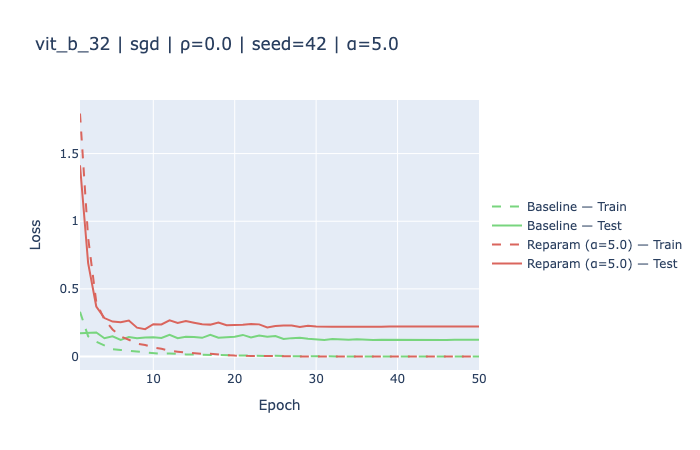
\includegraphics[width=0.48\textwidth]{./sgd_good.png} & 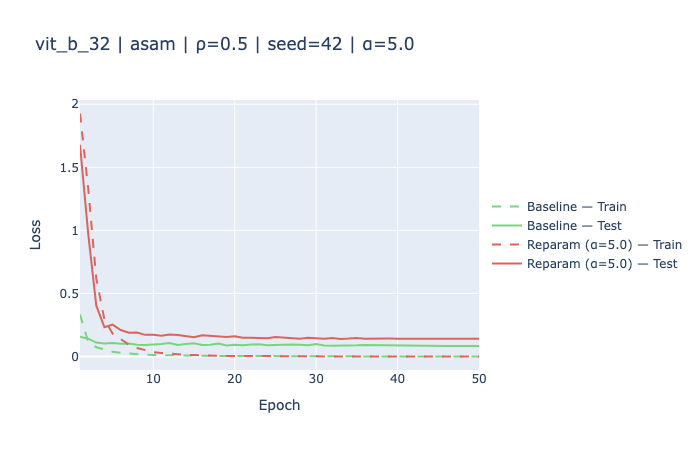
\includegraphics[width=0.48\textwidth]{./asam_good.png} \\
    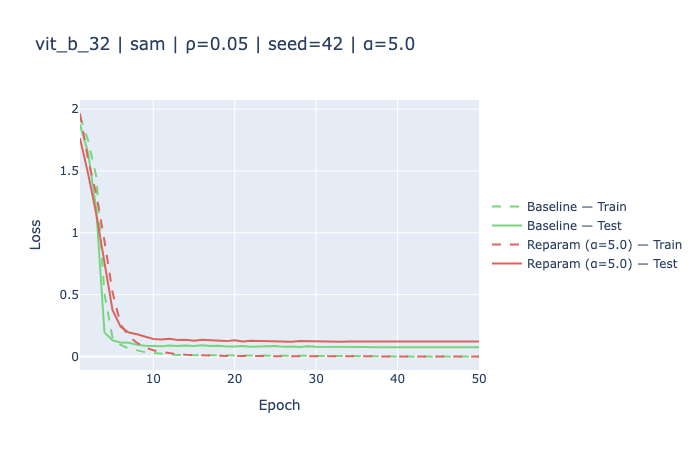
\includegraphics[width=0.48\textwidth]{./sam_good.png} & 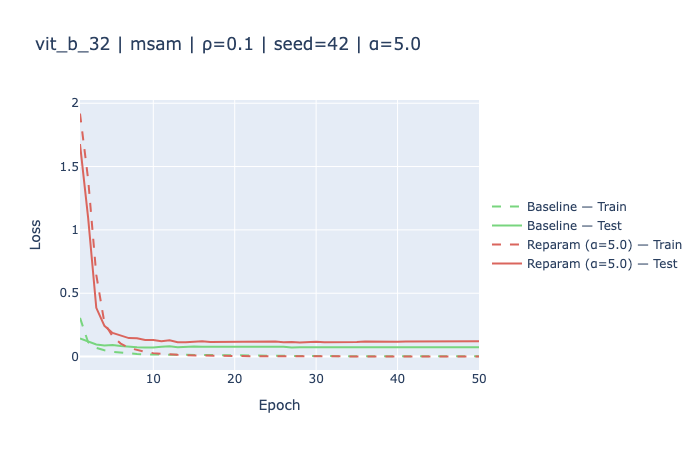
\includegraphics[width=0.48\textwidth]{./msam_good.png} \\
  \end{tabular}
    \caption{Epoch-wise training loss curves for ResNet-18 trained with SGD, SAM, ASAM, and M-SAM. The plot shows that M-SAM converges faster and achieves a lower training loss compared to the other optimizers, indicating its effectiveness in finding flatter minima.}
    \label{fig:sgd_good}
\end{figure}

\section{Contributions}
The contributions section is not included in the 5 page limit. This section should describe what each team member worked on and contributed to the project.

\section{Note on citations}

There are two citation commands:

\paragraph{Citation in parentheses} \verb|\citep{}| is for when you cite a paper at the end of a clause, and you could read the text out loud and not read the authors' names. For example ``We also run our experiments on a multilingual language model \citep{rajpurkar2018know}.'' 

\paragraph{Citation in text} \verb|\citet{}| is for in-text citations, when someone reading the text out loud would have to read the names of the authors for the sentence to make sense. For example, ``We also run our experiments on the multilingual model described in \citet{rajpurkar2018know}.''

\bibliographystyle{acl_natbib}
\bibliography{references}

\end{document}
